
%(BEGIN_QUESTION)
% Copyright 2010, Tony R. Kuphaldt, released under the Creative Commons Attribution License (v 1.0)
% This means you may do almost anything with this work of mine, so long as you give me proper credit

Identify whether the lead/lag function block needs to be configured for {\it lead} behavior or for {\it lag} behavior, based on the open-loop (i.e. control valve fixed at one position) step-change responses shown below, and also explain your answer in detail:

$$\includegraphics[width=15.5cm]{i04511x01.eps}$$


\vskip 20pt \vbox{\hrule \hbox{\strut \vrule{} {\bf Suggestions for Socratic discussion} \vrule} \hrule}

\begin{itemize}
\item{} Explain why it is critically important that the natural gas control valve {\it not move} during these tests.
\item{} Explain the significance of the ``+'' and ``$-$'' symbols next to the summer input lines.  How well would the system work if both of these inputs were non-inverting (``$+$'')?
\item{} How would this control system function if the summer function were moved to a location between the TT and TC?
\item{} How would this control system function if the lead/lag function were moved to a location between the TT and TC?
\item{} How would this control system function if the lead/lag function were moved to a location between the summer and the control valve?
\end{itemize}

\underbar{file i04511}
%(END_QUESTION)





%(BEGIN_ANSWER)

If your problem-solving included the thought, {\it ``We need to speed up the feed temperature's effect to bring it into step with the valve's effect''} then you have made a very common mistake.  I will leave it to you to determine why it is impossible for us to speed up the feed temperature's effect on the process using dynamic compensation in the control system.

%(END_ANSWER)





%(BEGIN_NOTES)

The function block needs to be configured for {\it lag} behavior, to help slow down the relatively fast response of the fuel gas's effect to match the feed temperature's effect on outlet temperature.

\vskip 10pt

From a comparison of the two lags seen on the trend graphs, we see that the compensation (fuel valve) has a faster effect on discharge temperature than the load (feed temperature).  Thus, in order to equalize the lags of these two effects, we need to slow down (lag more) the valve's compensating action.

%INDEX% Control, strategies: feedforward with dynamic compensation (lead/lag)

%(END_NOTES)


